\documentclass[11pt,pdftex,portrait,letterpaper]{article}
\usepackage[hdivide={1in,*,1in},
vdivide={1in,*,1in},
%            showframe
]{geometry}

% Standard packages
\usepackage[T1]{fontenc}
\usepackage{graphicx}
\usepackage{longtable}
\usepackage{acronym}
\usepackage{verbatim}
\usepackage{subfigure}
\usepackage{fancyhdr}
\pagestyle{fancy}
\usepackage{listings}
\usepackage{color}
\usepackage{lastpage}
\usepackage{caption}

% Fonts
%\usepackage{libertine}	% Libertine (the main font)
%\usepackage[lcgreekalpha]{libertinust1math}	% Libertine (as the math font)
\usepackage[varl]{inconsolata}	% A monospace font similar to Consolas. The varl option makes the lowercase l look different than a numeral 1.

% Last packages
\usepackage[hidelinks]{hyperref}	% Hyperlinks

% Modify parameters of Listings
\definecolor{lstgreen}{rgb}{0,0.6,0}
\definecolor{lstgray}{rgb}{0.4,0.4,0.4}
\lstset{ 
	language=C,
	basicstyle=\ttfamily\scriptsize,
	numbers=left,
	numberstyle=\footnotesize,
	keywordstyle=\color{blue},
	identifierstyle=\color{black},
	commentstyle=\color{lstgreen},
	stringstyle=\color{lstgray},
	stepnumber=1,
	numbersep=10pt,
	backgroundcolor=\color{white},
	frame=single,
	captionpos=b,
	breaklines=true,
	breakatwhitespace=false,
	tabsize=2,
	showstringspaces=false
}

% Default margins are too wide all the way around. Reset them here
\setlength{\topmargin}{-.5in}
\setlength{\textheight}{9in}
\setlength{\oddsidemargin}{0in}
\setlength{\textwidth}{6.5in}

\lhead{ECEN 220}
\chead{Timer/Counter Project 3}
\rhead{\thepage\ of \pageref{LastPage}}
\lfoot{\small{University of Nebraska--Lincoln}}
\cfoot{}
\rfoot{\small{Department of Electrical \& Computer Engineering}}
\renewcommand{\footrulewidth}{0.5pt}




\begin{document}
	
	\vspace*{30ex}
	\begin{center}
		
		\textbf{Timer/Counter Project 3}\\
		
		\vspace{4ex}
		ECEN 220: Introduction to Embedded Systems\\
		University of Nebraska--Lincoln\\
		March 6, 2021
		
		\vspace{4ex}
		Name: David Perez\\
		
	\end{center}
	
	
	\pagebreak
	\tableofcontents
	%\pagebreak
	%\listoffigures
	%\addcontentsline{toc}{section}{{\bf List of Figures}}
	\pagebreak
	
	
	\section{Introduction}
	
	
	For this project we were tasked to experiment with Pulse Width Modulations(PWM) that are made possible with the Arduino nanos. For the specific programs in this report, the fast PWM was used rather than the several others capable on the Arduino nanos. Using the fast PWM we were able to create a waveform of our choice and change the duty cycle as well. We were able to do this by simply changing the high time value in the OCR1A registers which changed how long the pin would be high for.
	
	Another useful opportunity that the PWM creates is it allows us to change the direction of servo motors. By adjusting the high time on our pulse wave we were able to rotate the servo clockwise or counterclockwise. On top of this, we used delays as well as the push botton to allow us to manualy change the motor direction. 	
	

	\section{Program Description}
	
	As stated in the introduction, both of the programs in this project use the fast PWM mode on the Arduino nanos. The period that we were aiming for is 20ms (that is 20ms from rising edge to rising edge). In program 1 we first initialized all of the register values and their corresponding addresses. Unfortunatley, the system clock runs far too fast for use to create the the high times that would later be needed in program 2. To get around this, I divided the system clock by a prescalar value of 8. This was derived by the following formula : Prescalar >= F(MCU)/( F(desired) * 40000)
	
	We were also tasked to selectively change the duty cycle which, for convenience, we used the ICR1H and ICR1L registers to change the TOP value of our PWM. we were able to achieve a 20ms period by also changing OCR1AH and OCR1AL registers which determined the high time our PWM. For my project I selected a TOP value of 40,000 and a high time of 10,000 (for 25\% duty cycle). The equation that was used to derive this is as follows:		100\% * (OCRIA / ICR1)
	
	Moving onto program 2, our objective was to use this wave form and adjust it to suit our servo motors. Using the a good portion of the information from program 1, we had to then create a wave form that had a high time in the range of 700-1500 microseconds for a clockwise rotation and a high time in the range of 1500-2300 microseconds for a counterclockwise rotation. On top of that, we then attached a push button to pin PB0 and when that value was debounced to 0 we would rotate the servo in one of the directions. A side note on that is we also had to make the motor stop and return to its original position after another press had occured and to make sure the motor woldn't prematurely rotate until the rotation had been complete.
	
	
		
	\subsection{Program 1}
	
	When creating this program there were a few important things to keep in mind. The first of which is the prescalar value that we chose. By using the formula mentioned above, I determined that if i wanted a frequency of 50Hz (period of 20ms) then I wouldn't be able to have a prescalar higher than 256 (as well as a prescalar lower that 8). The prescalar I chose was 8 which resulted in me having to assign a value of 40,000 for my ICR1 register. For the TCCR1A and TCCR1B registers, I assigned a value of 0b10 for COMIA to put PB1 in non-inverting mode, a value of 0b1110 for fast PWM mode with a TOP value dependent on ICR1A and a value of 0b010 for CS1 to divide my clock down by a prescalar of 8. With these values in place I was thus able to obtain a duty cycle of 25\%, 50\% and 75\%.
	Below are images that display the different duty cycles that were generated and thus read using a logic analyzer.
\pagebreak
	\begin{figure}[h]
		\centering
		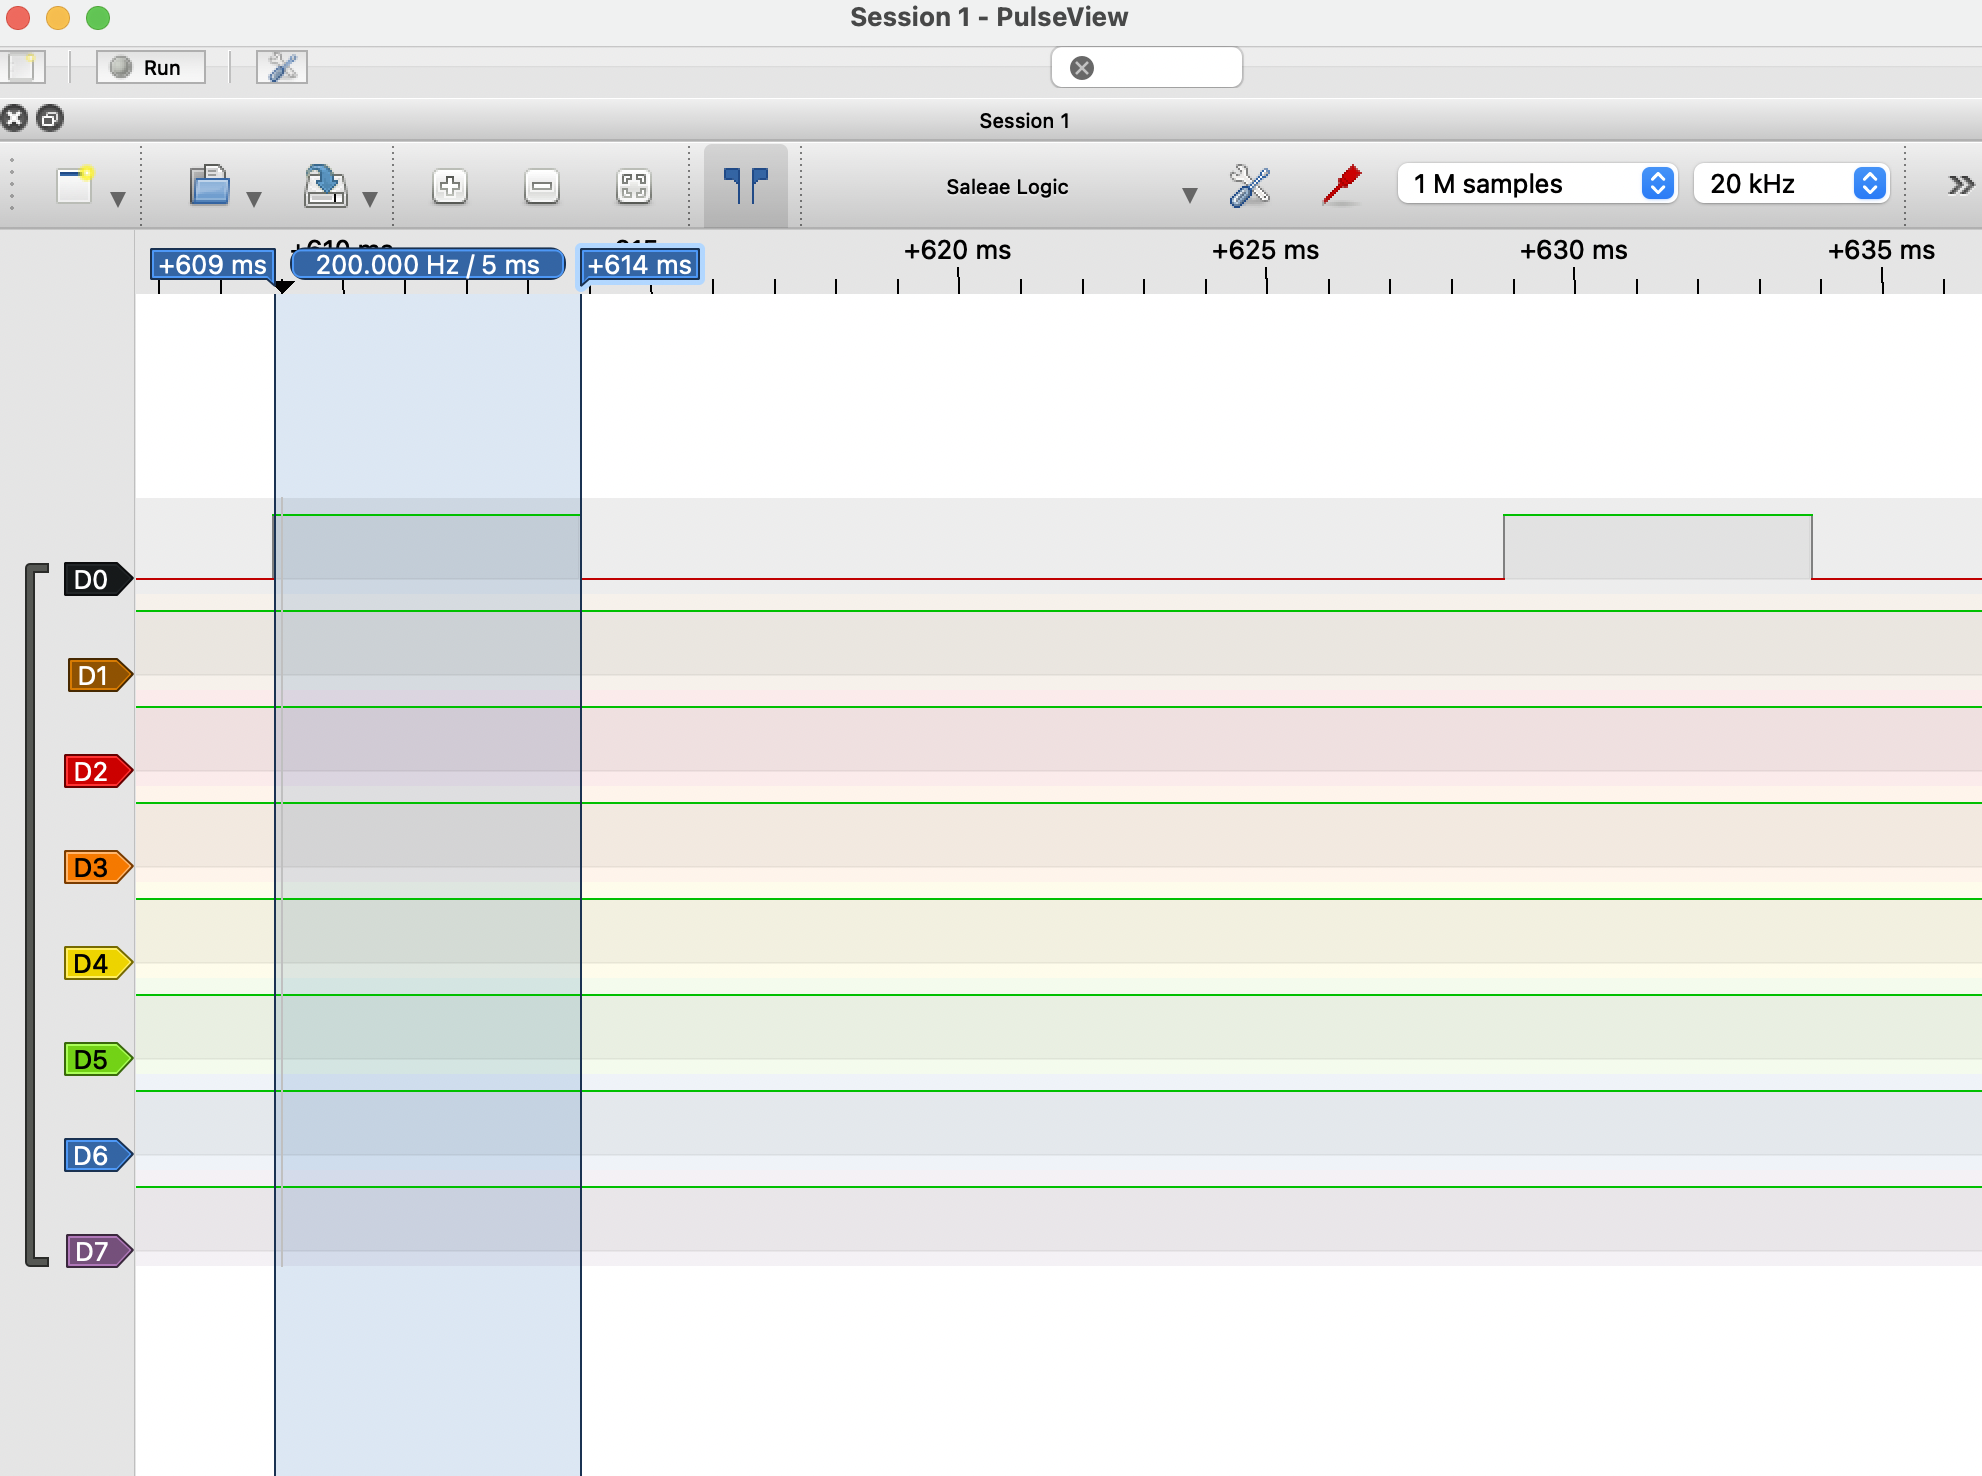
\includegraphics[width=0.37\textwidth]{./proj3_25DS}	% The .png file will be used to make the figure here, and is in the same directory as this .tex file
		\caption{Screen Capture a 25\% duty cycle}
		\label{f:fig1}	% labels must come after the caption
	\end{figure}
	\begin{figure}[h]
	\centering
	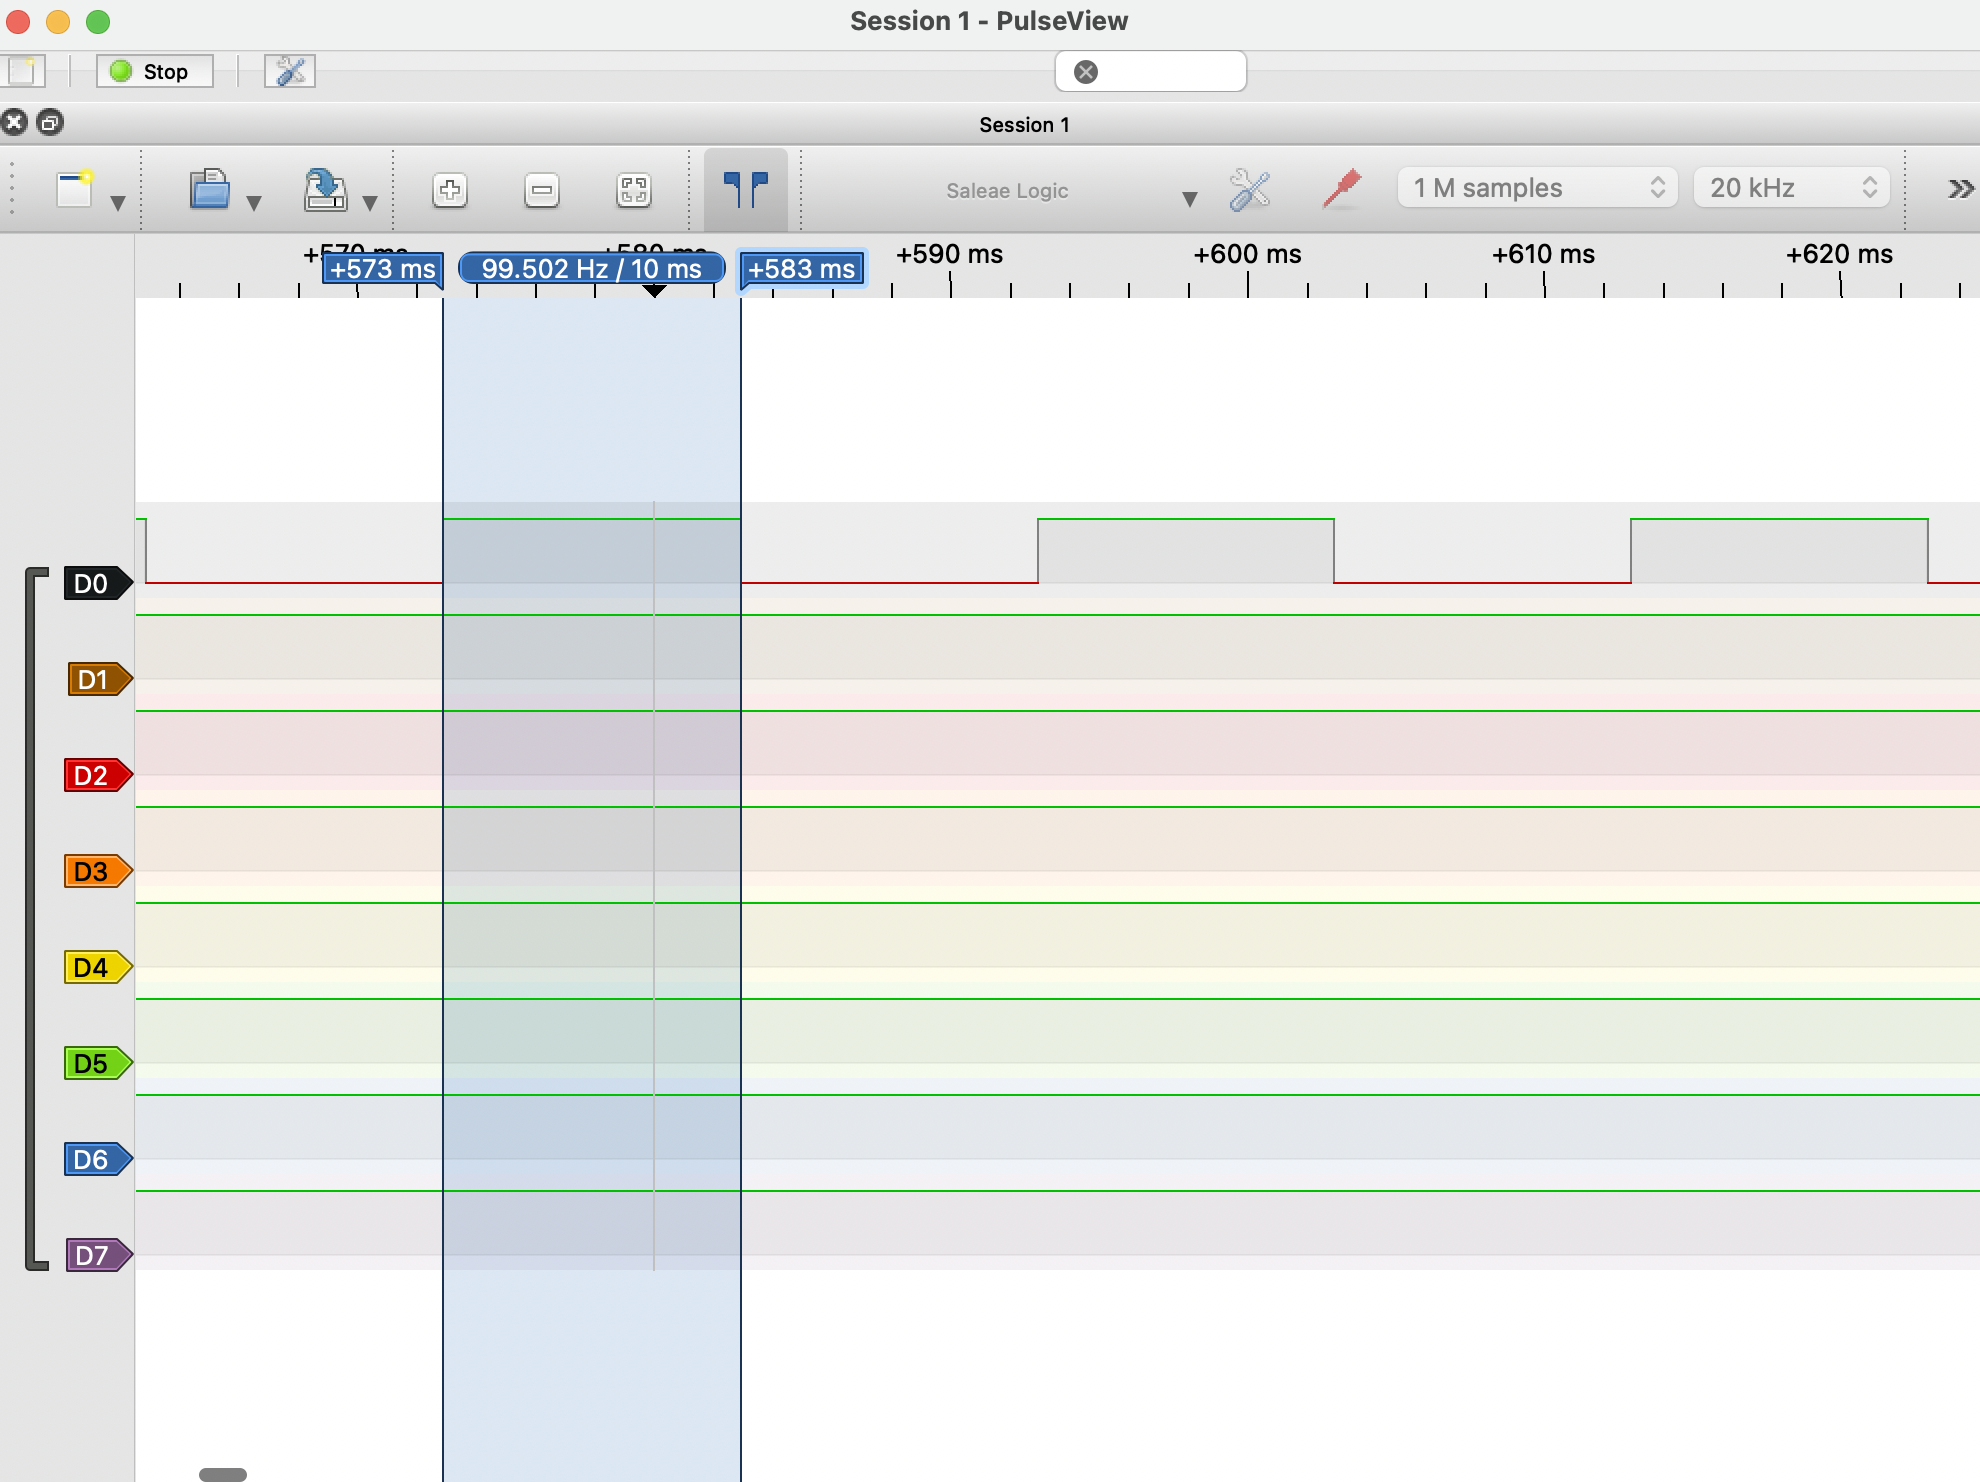
\includegraphics[width=0.37\textwidth]{./proj3_50DS}	% The .png file will be used to make the figure here, and is in the same directory as this .tex file
	\caption{Screen Capture a 50\% duty cycle}
	\label{f:fig1}	% labels must come after the caption
	\end{figure}
	\begin{figure}[h]
	\centering
	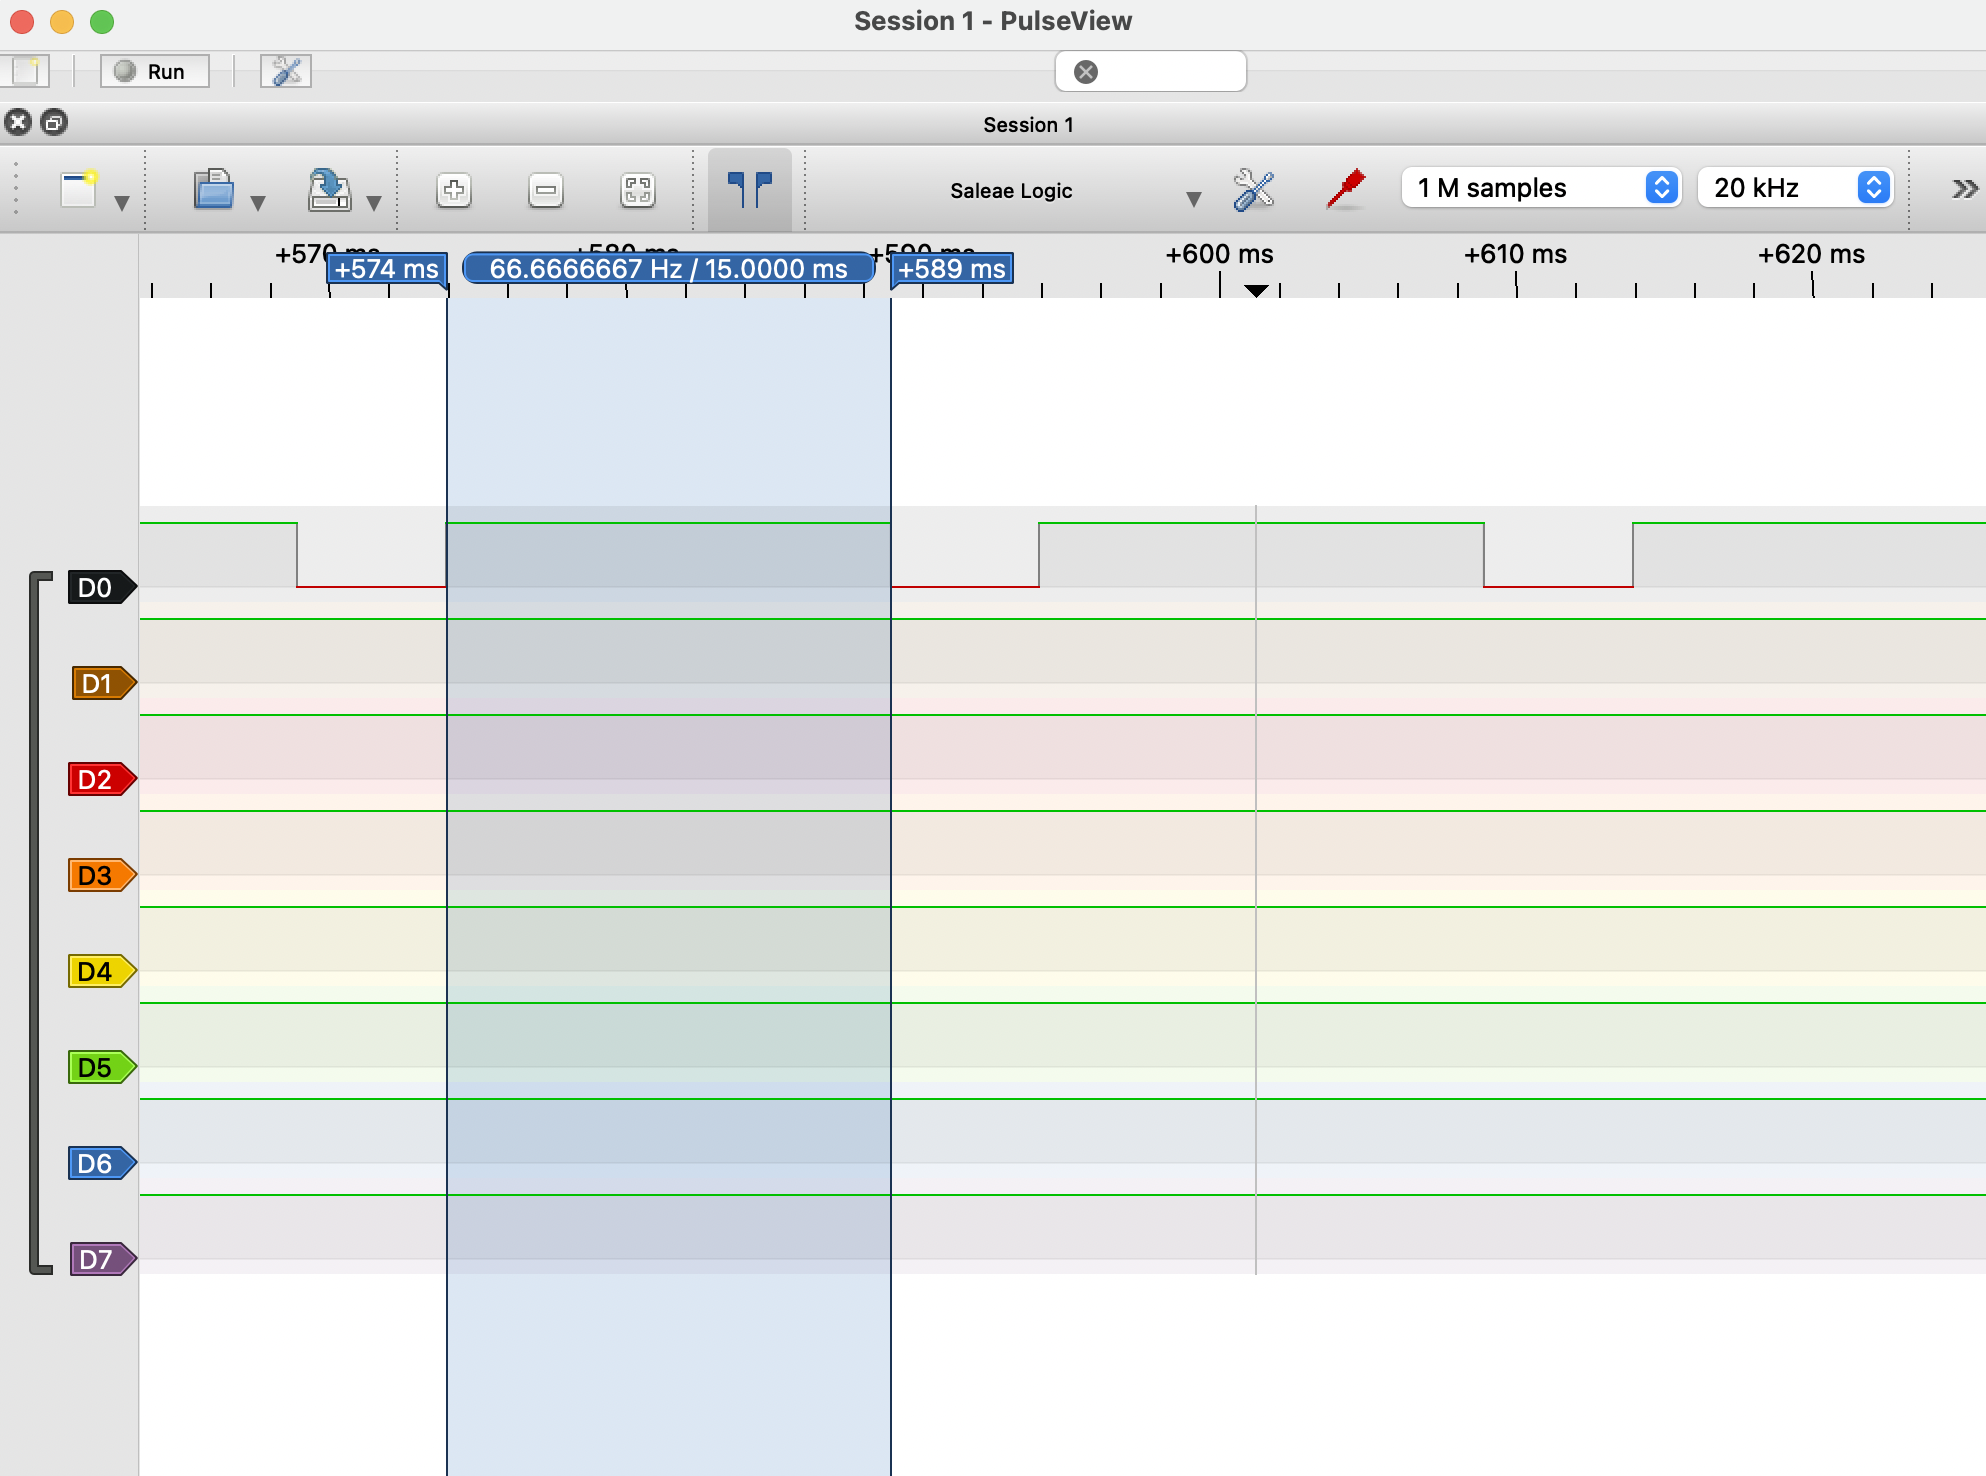
\includegraphics[width=0.37\textwidth]{./proj3_75DS}	% The .png file will be used to make the figure here, and is in the same directory as this .tex file
	\caption{Screen Capture a 75\% duty cycle}
	\label{f:fig1}	% labels must come after the caption
	\end{figure}
\pagebreak

	
	
	\subsection{Program 2}

	For program 2, we are using the waveform from program 1 but trimming down our high time to suit our servo motor direction specifications that would be controlled by a pushbutton. To construct this program there was several things to keep in mind. After establishing all the initial register values I then had to construct the logic that would enable the servo to respond to the button presses. First off, I had to debounce the button to make sure I wasn't getting garbage values when reading the pin (PB0) that the button was connected to. Once I did this and detected a state change I then had to decide if the button was being pressed or not. If all these came out to be true and a button had been pressed I could then decide which direction to turn the motor. I accomplished this by using a flag to remember the previous direction the motor had rotated. Based on this value I rotated the servo in the desired direction. A value of 2250 was assigned to OCR1A to rotate the servo clockwise and 3800 to rotate the motor counterclockwise.
	
	The period for this program remained the same throughout but the high time and duty cycle changed between based on one of the two values assigned to OCR1A. When rotating clockwise, the duty cycle came out to 5.625\% which is pictured in Figure 4 below.
		\begin{figure}[h]
		\centering
		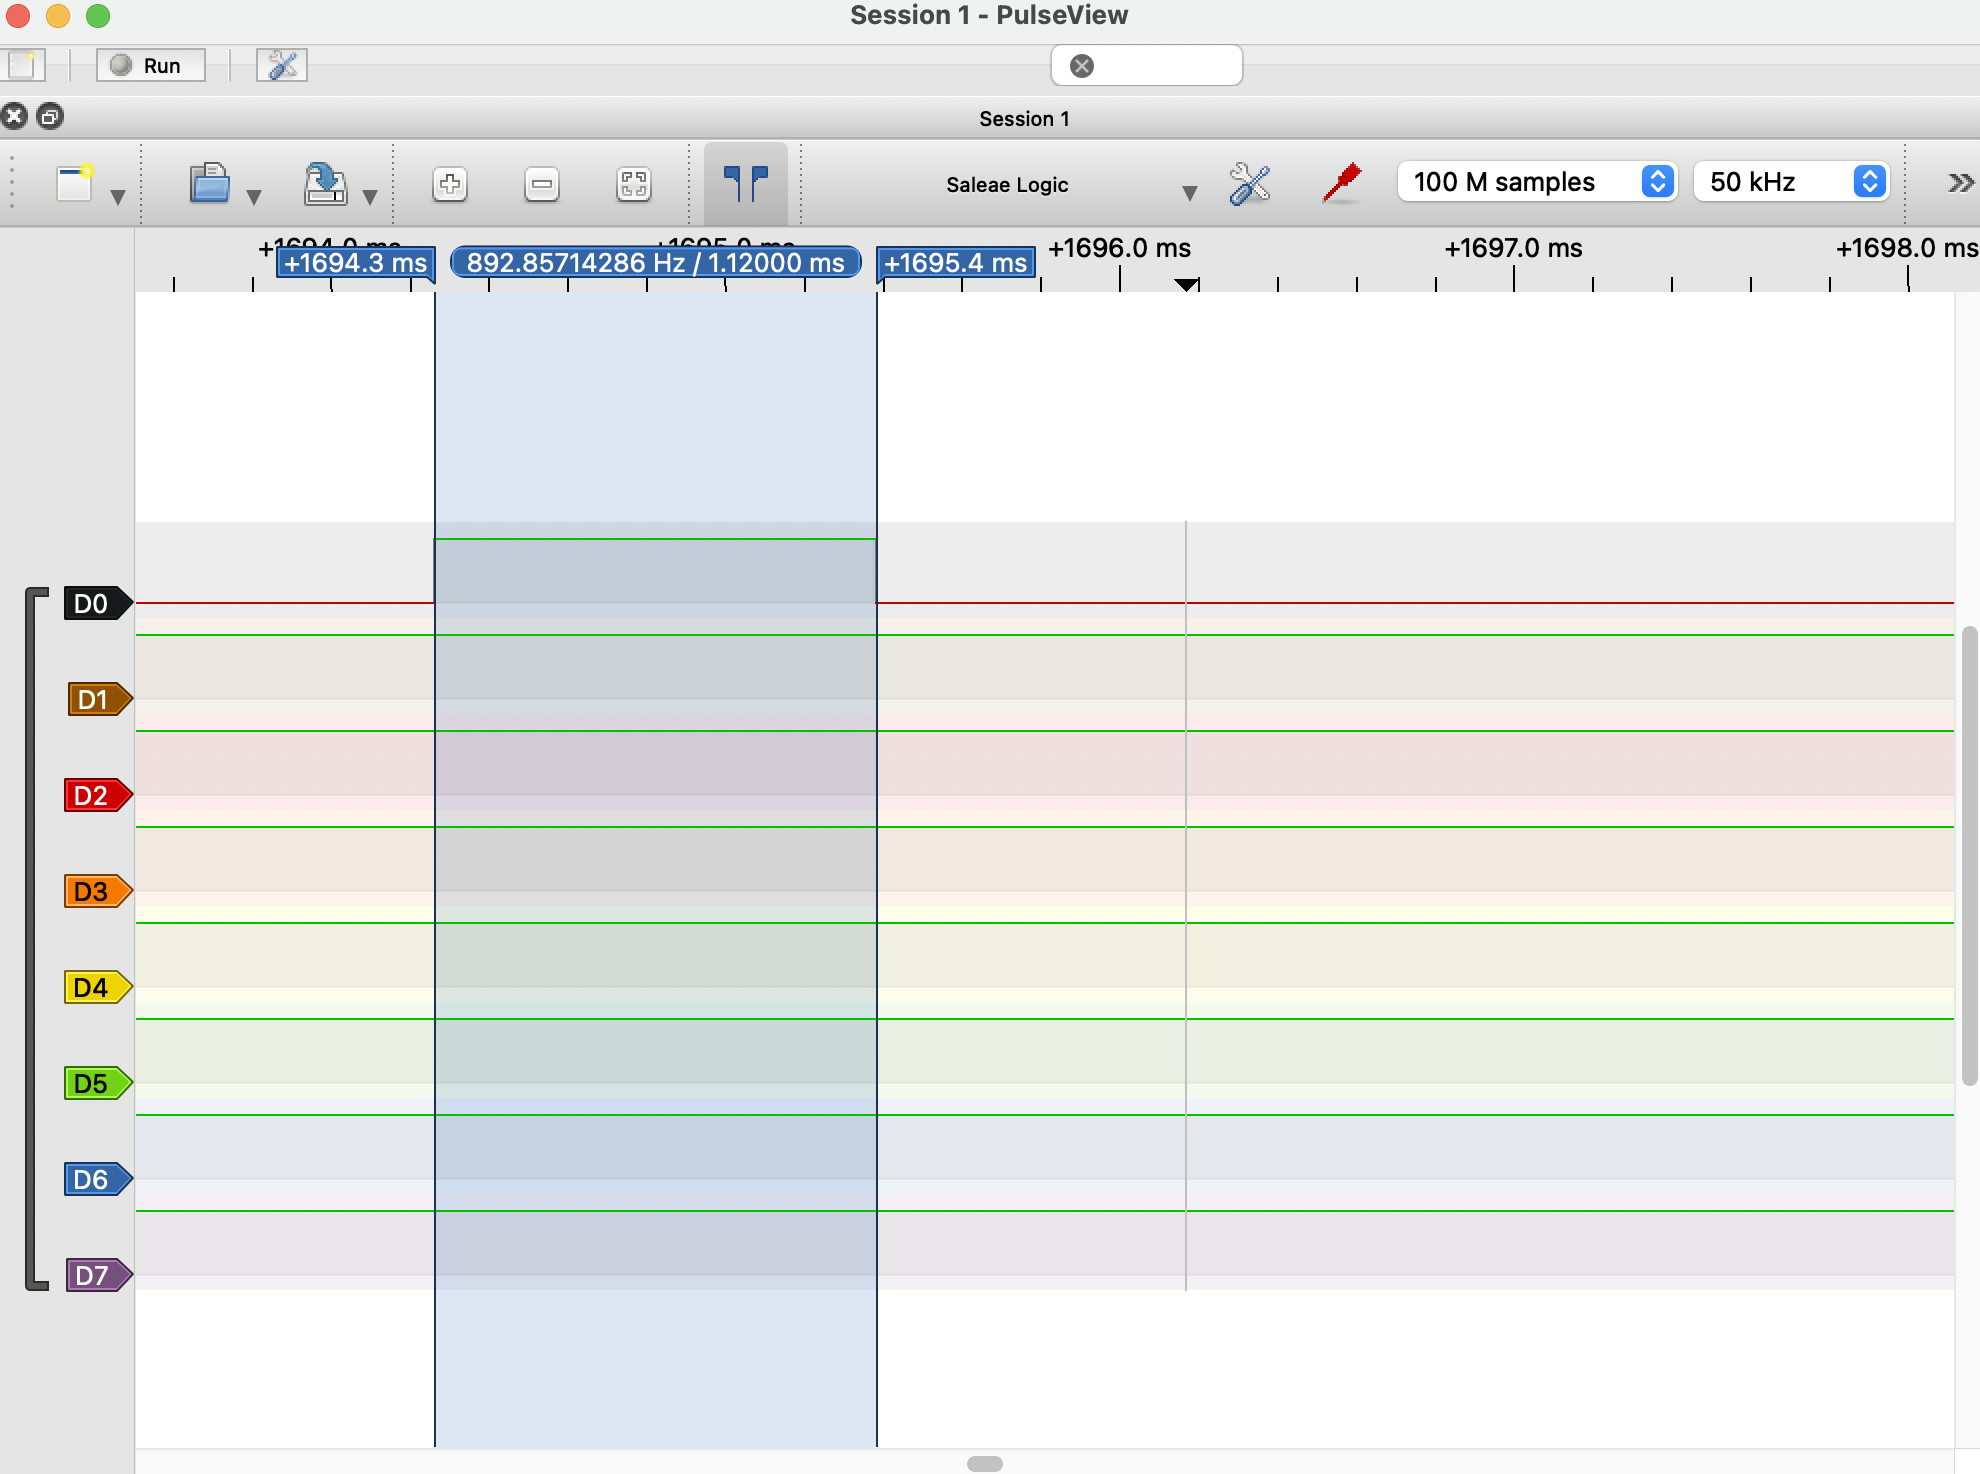
\includegraphics[width=0.37\textwidth]{./program2_clockwise}	% The .png file will be used to make the figure here, and is in the same directory as this .tex file
		\caption{Servo Rotating Clockwise with a 5.625\%duty cycle}
		\label{f:fig1}	% labels must come after the caption
	\end{figure}
	
	When rotating the servo counterclockwise the duty cyle came out to be 9.5\%. This is pictured below in Figure 5.
	\begin{figure}[h]
		\centering
		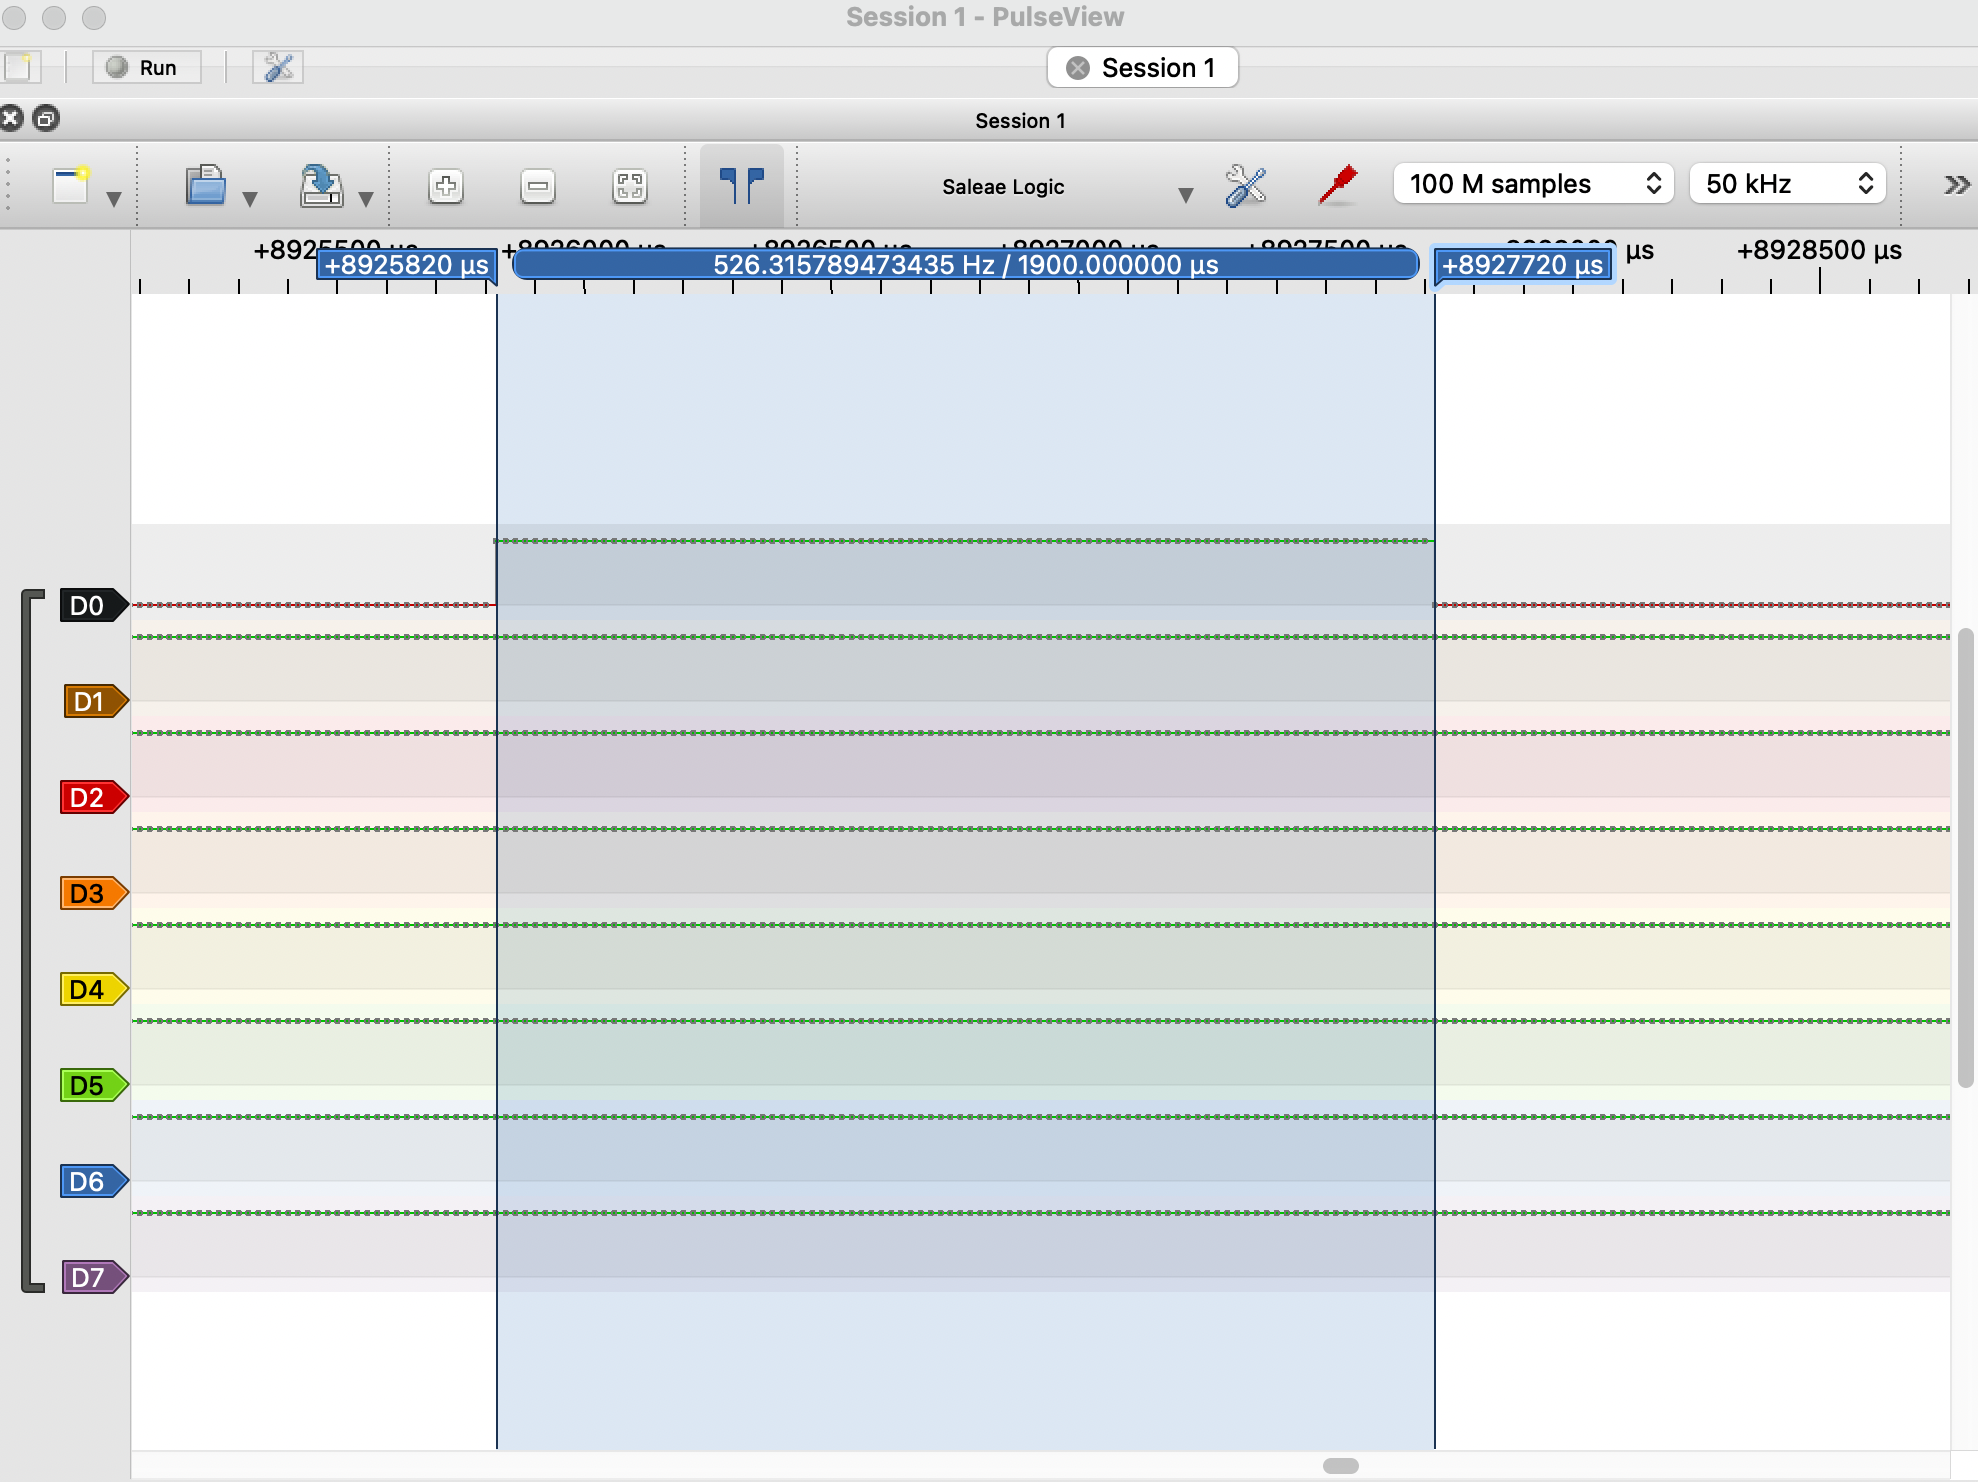
\includegraphics[width=0.37\textwidth]{./program2_counterclockwise}	% The .png file will be used to make the figure here, and is in the same directory as this .tex file
		\caption{Servo Rotating Clockwise with a 9.5\%duty cycle}
		\label{f:fig1}	% labels must come after the caption
	\end{figure}
	
	When the motor was not turning the duty cycle would thus be \%. The reason behind this was because in order to stop the motor from rotating I had assigned a 0 as the high time in the OCR1A register which meant that the pin would never be high when it wasn't rotating. This is visually depicted in Figure 6 below.
		\begin{figure}[h]
		\centering
		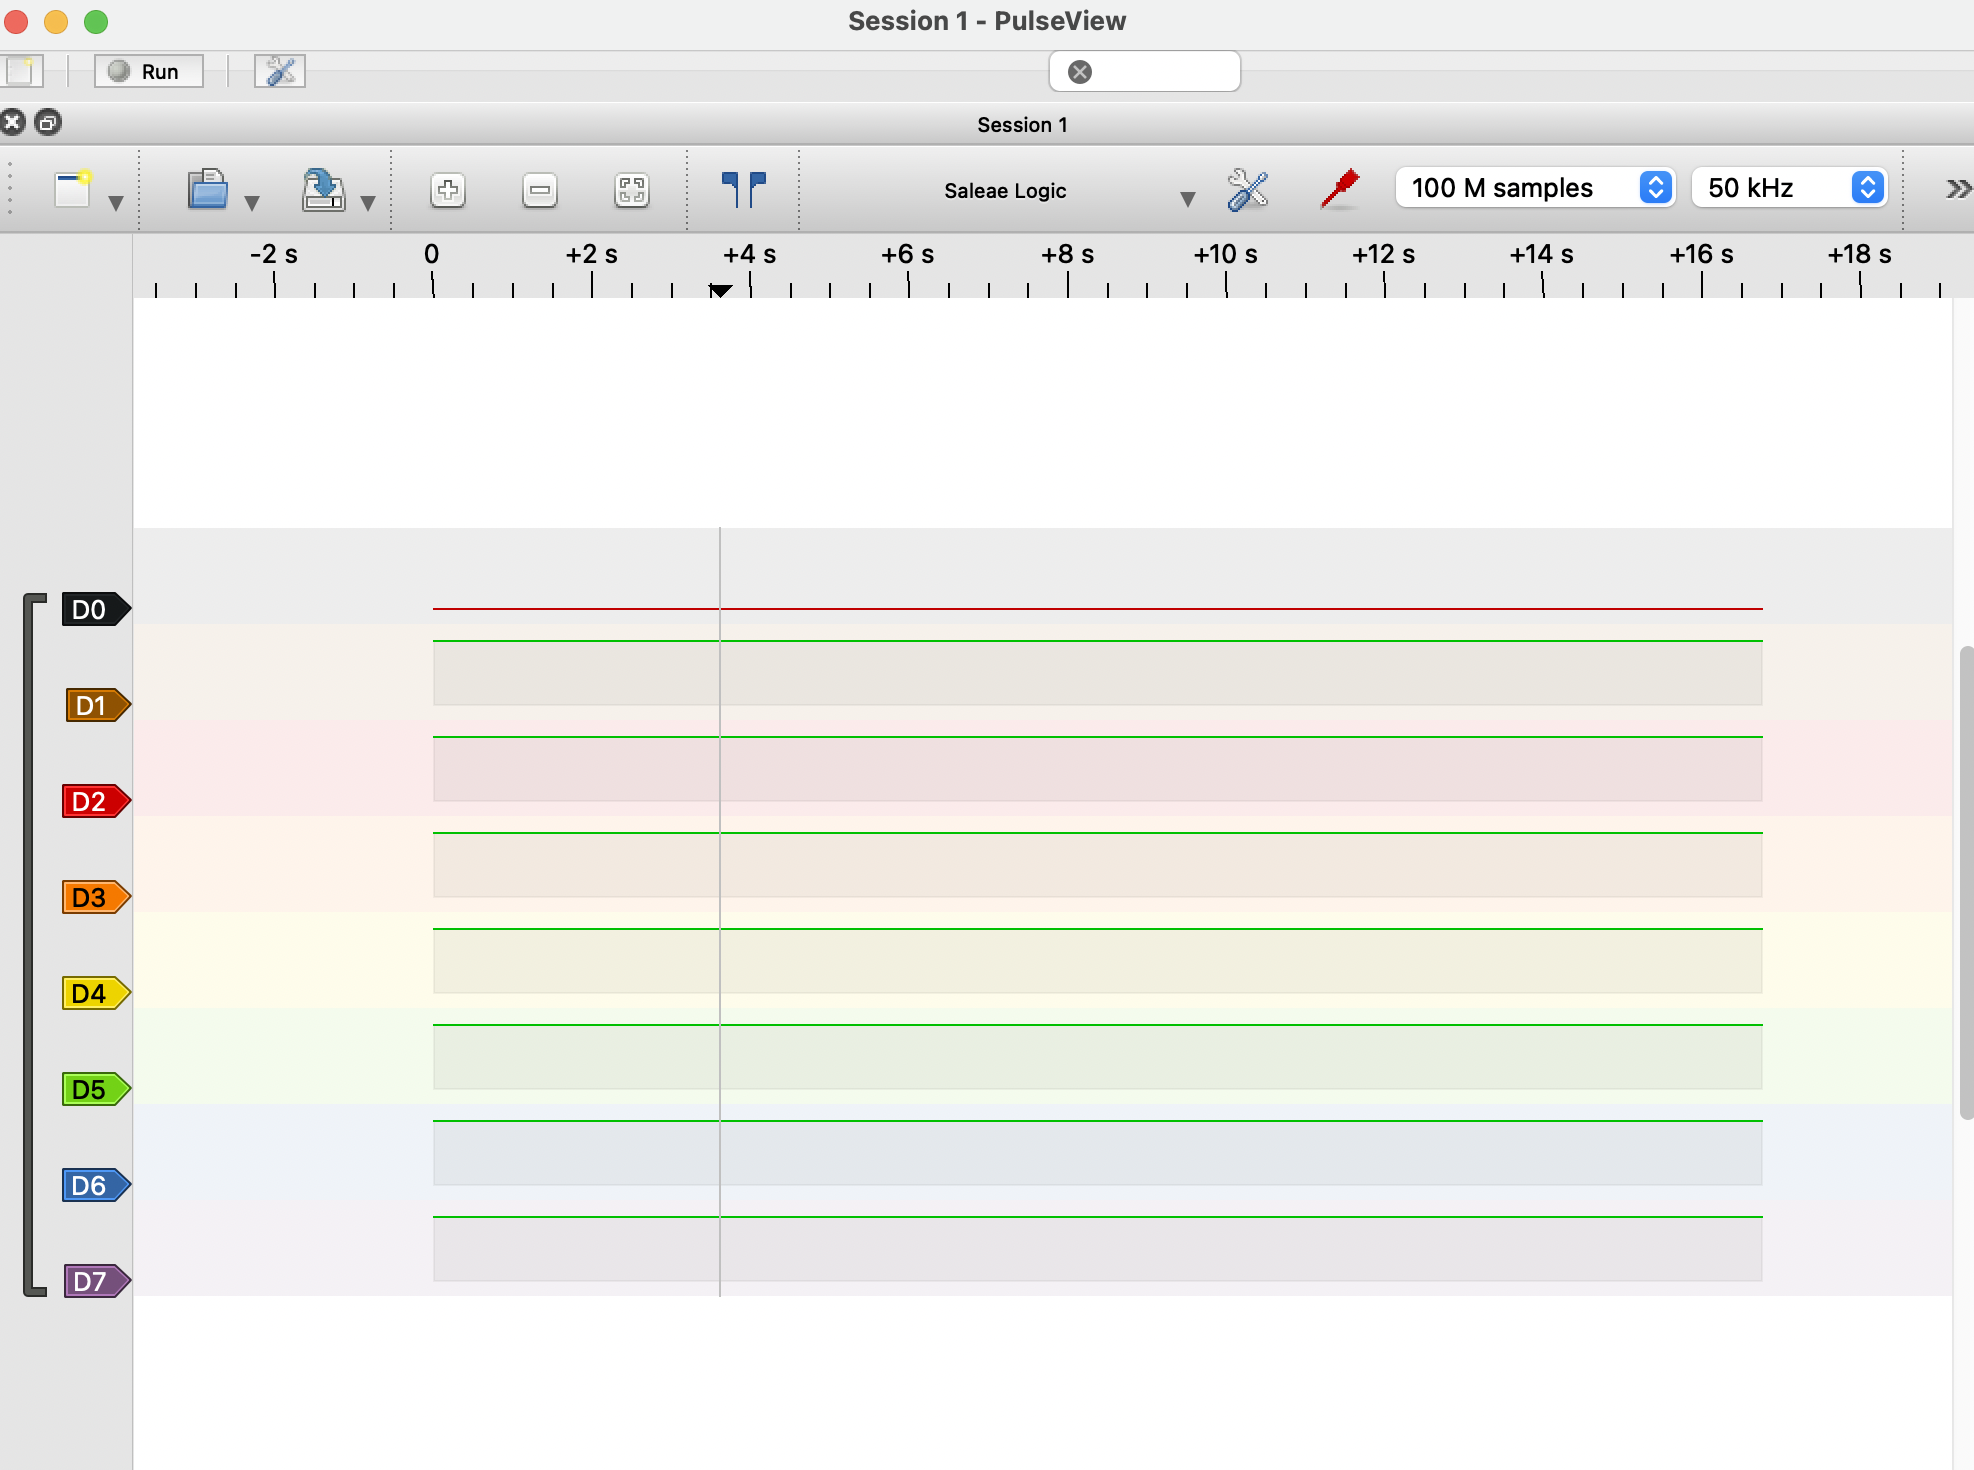
\includegraphics[width=0.37\textwidth]{./program2_noRotations}	% The .png file will be used to make the figure here, and is in the same directory as this .tex file
		\caption{Servo idle with 0\% duty cycle}
		\label{f:fig1}	% labels must come after the caption
	\end{figure}

	Lastly I would like to talk about the power that is being used by the servo motor when the motor is in motion and when it is not. To calculate this I mutliplied the meausured Arduino nano voltage of 4.74 by the current being drawn from the motor. When the motor is idle it draws roughly 18 milli-watts(mW) of power. When in motion, the motor draws significantly more power in the range of 40mW to about 150mW. I included a table below because the power drawn can be very inconsistent.
	
	\begin{table}[htb]
		\centering
		\begin{tabular}{ | c | c | c | c | }	% add more columns (r, c, or l for the justification) and column separators (|) here
			\hline
			\textbf{Measured Current of Moving Motor(mA)} & \textbf{Calculated Power(mW)}  \\ \hline \hline
			 140.4 & 665.5  \\ \hline
			52.5 & 248.85 \\ \hline
			88.5 & 419.49 \\ \hline
			103 & 488.22 \\ \hline
			142.5 & 675.45 \\ \hline	
			133.4 & 632.316 \\ \hline
			129.5 & 613.83 \\ \hline		
			93.2 & 441.77 \\ \hline				
		\end{tabular}
		\caption{Program 2 Current and Power Consumed by Motor in Motion }
		\label{t:table1}	% labels must come after the caption
	\end{table}

\pagebreak
	

	
	\section{Conclusion}
	

	
	Both programs in this project offered some very important information on waveforms. With program 1 we were able to grasp an understanding on how to create a PWM. By using the timer of the Arduino nano we were able to create these waveforms. From there we were able to use that information and generate waveforms of our choosing and even adjust the duty cycle of these waveforms. With that we were able to use this information and apply it to a very important component in electrical engineering and that is the electric motor. With our version of an electric motor, the servo motor, we were able to change its direction based on the high times of the wave form that we gave it. Then, with the help of a push button we could manually change the servo motors direction. All in all, we learned how to generate wave forms, change their duty cycles, and even apply this to an electric motor to get it to respond in the manner that we desired.
	
	

	
	\section{Appendix}
	
	%Here is an example of how to add good-looking code snippets using a 'listing' 
	\begin{lstlisting}[caption={Program 1}, label=l:programx]
	/** Includes **/
	#include <stdint.h>

	
	
	/** Memory mapped register defines **/
	#define REG_DDRB (*((volatile uint8_t*) 0x24))
	
	#define REG_TCCR1A (*((volatile uint8_t*) 0x80))
	#define REG_TCCR1B (*((volatile uint8_t*) 0x81))
	#define REG_OCR1AH (*((volatile uint8_t*) 0x89))
	#define REG_OCR1AL (*((volatile uint8_t*) 0x88))
	
	#define REG_ICR1H (*((volatile uint8_t*) 0x87))
	#define REG_ICR1L (*((volatile uint8_t*) 0x86))
	
	//Registers for debouncing function
	volatile uint8_t* pPINB;
	volatile uint8_t* pDDRB;
	volatile uint8_t* pPORTB;
	
	/** Function declarations **/
	int8_t debouncePin(volatile uint8_t* mmrPINx, uint8_t bitToRead);
	void myHardDelay(uint32_t delayInMsec);
	
	
	int main()
	{
		//assign register values to variables
		pPINB = 0x23;
		pDDRB = 0x24;
		pPORTB = 0x25;
		
		//Seting up registers for debouncing function
		// set PB0 as an input
		*pDDRB = 0x00;  //0b00000000
		
		// Set PB0 as having a internal pullup resistor enabled
		*pPORTB = (*pPORTB) | 0x01; //0b00000001
		/*
		Specifications:
		1.Output a square wave on pin OC1A, which is PB1
		2. Make the duty cycle customizable, and make it proportional to OCR1A / TOP (aka non-inverting mode)
		3. Use the fast PWM mode that sets the TOP value as ICR1A
		4. Use a Timer/counter 1 clock source of f_MCU / 1.
		Note: this will give a period of T = TOP * prescalar / f_MCU
		*/
		
		/*
		Determine bit fields
		WGM1[3:0] = 0B1110 for fast PWM mode where TOP = ICR1A 
		COM1A[1:0] = 0b10 for non-inverting mode on pin OCR1A / PB1
		
		// determine WHAT PRESCALAR AND ICR1A VALUE TO USE
		CS1[2:0] = 0b010 for a clock prescalar of / 8 
		Now our timer will increment every 8/16MHz = 5x10^(-7) 50 micosecond??
		*/
		
		//Set the registers for Fast PWM
		
		//Configure PB1 as an output
		REG_DDRB = 0x02;
		
		//TCCR1A contains COM1A[1:0] bit field and the WGM1[1:0] partial bit field.
		// COM1A[1:0] cat 0b0000 cat WGM1[1:0]= 0b10 == 0b10000010 == 0x82
		REG_TCCR1A = 0x82;
		
		//Configure the TOP value aka ICR1AH and ICR1AL
		uint16_t top_value = 40000;
		REG_ICR1H = top_value >> 8;
		REG_ICR1L = top_value & 0x00FF;
		
		//set a small high time to prevent the servo from moving once the TCCR1B register is initialized
		uint16_t high_time = 1;
		REG_OCR1AH = high_time >> 8;
		REG_OCR1AL = high_time & 0x00FF;
		
		//TCCR1B = 0b000 cat WGM1[3:2] cat CS1[2:0] == 0b000 cat 0b11 cat 0b010 == 00011010 == 0x1A
		REG_TCCR1B = 0x1A;
		
		//initialize flag for the servo direction where a 0 rotates clockwise and a 1 rotates counter clockwise
		int8_t servoDirection = 0;
		while(1)
		{
			//debounce the pushbutton
			int8_t state1 = debouncePin(0x23, 0x01);
			
			//check if the button is done bouncing 
			if(state1 == (-1) | state1 == 1)
			{
				int8_t state2 = *pPINB & 0x01;
				//check for a state change on PB0
				if(state1 != state2)
				{
					//check if the button is being pushed
					if(state1 == (-1))
					{
						//rotate the servo in a clockwise directoins
						if(servoDirection == 0)
						{
							
							for(volatile uint32_t z=0; z < 100000; z++)
							{
								high_time = 2250;
								REG_OCR1AH = high_time >> 8;
								REG_OCR1AL = high_time & 0x00FF;
							}
							high_time = 0;
							REG_OCR1AH = high_time >> 8;
							REG_OCR1AL = high_time & 0x00FF;
							//change the servo direction next time loop occurs
							servoDirection = 1;
						}
						
						//rotate the servo counterclockwise
						else if (servoDirection == 1)
						{
							for(volatile uint32_t j=0; j < 100000; j++)
							{
								high_time = 3800;
								REG_OCR1AH = high_time >> 8;
								REG_OCR1AL = high_time & 0x00FF;
							}
							high_time = 0;
							REG_OCR1AH = high_time >> 8;
							REG_OCR1AL = high_time & 0x00FF;
							
							///change the servo direction next time loop occurs
							servoDirection = 0;
						}
					}
				}
			}
		}
	}
	
	
	int8_t debouncePin(volatile uint8_t* mmrPINx, uint8_t bitToRead)
	{
		//read PB0
		uint8_t firstDebouceSample = *mmrPINx & bitToRead;
		
		//Delay for 30 milliseconds
		myHardDelay(30);
		
		uint8_t secondDebouceSample = *mmrPINx & bitToRead;
		
		if(firstDebouceSample == secondDebouceSample)
		{
			//The pin is successfully debounced
			if(firstDebouceSample == 0x00)
			{
				//The pin is being pushed (debounced and low)
				return -1;
			}
			else
			{
				// The pin is not being pushed (debounced and high)
				return 1;
			}
		}
		else{
			// The pin may be bouncing
			return 0;
		}
	}
	
	void myHardDelay(uint32_t delayInMsec)
	{
		volatile uint16_t delayCount;
		volatile uint16_t i;
		delayCount = delayInMsec * 373;
		for(i=0;i <delayCount; i++){
			
		}
	}
	\end{lstlisting}
	
	\begin{lstlisting}[caption={Program 2}, label=l:programx]
	/** Includes **/
	#include <stdint.h>

	
	
	/** Memory mapped register defines **/
	#define REG_DDRB (*((volatile uint8_t*) 0x24))
	
	#define REG_TCCR1A (*((volatile uint8_t*) 0x80))
	#define REG_TCCR1B (*((volatile uint8_t*) 0x81))
	#define REG_OCR1AH (*((volatile uint8_t*) 0x89))
	#define REG_OCR1AL (*((volatile uint8_t*) 0x88))
	
	#define REG_ICR1H (*((volatile uint8_t*) 0x87))
	#define REG_ICR1L (*((volatile uint8_t*) 0x86))
	
	/** Function declarations **/
	void myHardDelay(uint32_t delayInMsec);
	
	
	int main()
	{
		/*
		Specifications:
		1.Output a square wave on pin OC1A, which is PB1
		2. Make the duty cycle customizable, and make it proportional to OCR1A / TOP (aka non-inverting mode)
		3. Use the fast PWM mode that sets the TOP value as ICR1A
		4. Use a Timer/counter 1/8 clock source of f_MCU / 8.
		Note: this will give a period of T = TOP * prescalar / f_MCU
		*/
		
		
		/*
		Determine bit fields
		WGM1[3:0] = 0B1110 for fast PWM mode where TOP = ICR1A 
		COM1A[1:0] = 0b10 for non-inverting mode on pin OCR1A / PB1
		
		// determine WHAT PRESCALAR AND ICR1A VALUE TO USE
		CS1[2:0] = 0b010 for a clock prescalar of / 8 
		Now our timer will increment every 8/16MHz = 5x10^(-7) 50 micosecond??
		*/
		
		//Set the registers
		
		//Configure PB1 as an output
		REG_DDRB = 02;
		
		//TCCR1A contains COM1A[1:0] bit field and the WGM1[1:0] partial bit field.
		// COM1A[1:0] cat 0b0000 cat WGM1[1:0]= 0b10 == 0b10000010 == 0x82
		REG_TCCR1A = 0x82;
		
		//Configure the TOP value aka ICR1AH and ICR1AL
		uint16_t top_value = 40000;
		REG_ICR1H = top_value >> 8;
		REG_ICR1L = top_value & 0x00FF;
		
		// Set the initial duty cycle to 25%. Do this before the timer is turned on,
		//which happens when CS1 is no longer 0b000 (this is
		//done when TCCR1B is configured, so do it before then!)
		
		uint16_t high_time = 10000; //to create a 25% duty cycle
		/* uint16_t high_time = 20000; //to create a 50% duty cycle
		uint16_t high_time = 30000; // to create a 75% duty cycle */
		
		REG_OCR1AH = high_time >> 8;
		REG_OCR1AL = high_time & 0x00FF;
		
		//TCCR1B = 0b000 cat WGM1[3:2] cat CS1[2:0] == 0b000 cat 0b11 cat 0b010 == 00011010 == 0x1A
		REG_TCCR1B = 0x1A;
		
		
		//continuously cycle the fast PWM 
		while(1)
		{
			high_time = 10000;
			REG_OCR1AH = high_time >> 8;
			REG_OCR1AL = high_time & 0x00FF;
		}
	}
	
	void myHardDelay(uint32_t delayInMsec)
	{
		volatile uint16_t delayCount;
		volatile uint16_t i;
		delayCount = delayInMsec * 373;
		for(i=0;i <delayCount; i++){
		}
	}
		
	\end{lstlisting}
	

	
	
\end{document}



